\documentclass{article}
\usepackage[margin=1in]{geometry}
\usepackage[linesnumbered,ruled,vlined]{algorithm2e}
\usepackage{amsfonts}
\usepackage{amsmath}
\usepackage{amssymb}
\usepackage{amsthm}
\usepackage{enumitem}
\usepackage{fancyhdr}
\usepackage{hyperref}
\usepackage{minted}
\usepackage{multicol}
\usepackage{pdfpages}
\usepackage{standalone}
\usepackage[many]{tcolorbox}
\usepackage{tikz-cd}
\usepackage{transparent}
\usepackage{xcolor}
% \tcbuselibrary{minted}

\author{Nathan Solomon}

\newcommand{\fig}[1]{
    \begin{center}
        \includegraphics[width=\textwidth]{#1}
    \end{center}
}

% Math commands
\renewcommand{\d}{\mathrm{d}}
\DeclareMathOperator{\id}{id}
\DeclareMathOperator{\im}{im}
\DeclareMathOperator{\proj}{proj}
\DeclareMathOperator{\Span}{span}
\DeclareMathOperator{\Tr}{Tr}
\DeclareMathOperator{\tr}{tr}
\DeclareMathOperator{\ad}{ad}
\DeclareMathOperator{\ord}{ord}
%%%%%%%%%%%%%%% \DeclareMathOperator{\sgn}{sgn}
\DeclareMathOperator{\Aut}{Aut}
\DeclareMathOperator{\Inn}{Inn}
\DeclareMathOperator{\Out}{Out}
\DeclareMathOperator{\stab}{stab}

\newcommand{\N}{\ensuremath{\mathbb{N}}}
\newcommand{\Z}{\ensuremath{\mathbb{Z}}}
\newcommand{\Q}{\ensuremath{\mathbb{Q}}}
\newcommand{\R}{\ensuremath{\mathbb{R}}}
\newcommand{\C}{\ensuremath{\mathbb{C}}}
\renewcommand{\H}{\ensuremath{\mathbb{H}}}
\newcommand{\F}{\ensuremath{\mathbb{F}}}

\newcommand{\E}{\ensuremath{\mathbb{E}}}
\renewcommand{\P}{\ensuremath{\mathbb{P}}}

\newcommand{\es}{\ensuremath{\varnothing}}
\newcommand{\inv}{\ensuremath{^{-1}}}
\newcommand{\eps}{\ensuremath{\varepsilon}}
\newcommand{\del}{\ensuremath{\partial}}
\renewcommand{\a}{\ensuremath{\alpha}}

\newcommand{\abs}[1]{\ensuremath{\left\lvert #1 \right\rvert}}
\newcommand{\norm}[1]{\ensuremath{\left\lVert #1\right\rVert}}
\newcommand{\mean}[1]{\ensuremath{\left\langle #1 \right\rangle}}
\newcommand{\floor}[1]{\ensuremath{\left\lfloor #1 \right\rfloor}}
\newcommand{\ceil}[1]{\ensuremath{\left\lceil #1 \right\rceil}}
\newcommand{\bra}[1]{\ensuremath{\left\langle #1 \right\rvert}}
\newcommand{\ket}[1]{\ensuremath{\left\lvert #1 \right\rangle}}
\newcommand{\braket}[2]{\ensuremath{\left.\left\langle #1\right\vert #2 \right\rangle}}

\newcommand{\catname}[1]{{\normalfont\textbf{#1}}}

\newcommand{\up}{\ensuremath{\uparrow}}
\newcommand{\down}{\ensuremath{\downarrow}}

% Custom environments
\newtheorem{thm}{Theorem}[section]

\definecolor{probBackgroundColor}{RGB}{250,240,240}
\definecolor{probAccentColor}{RGB}{140,40,0}
\newenvironment{prob}{
    \stepcounter{thm}
    \begin{tcolorbox}[
        boxrule=1pt,
        sharp corners,
        colback=probBackgroundColor,
        colframe=probAccentColor,
        borderline west={4pt}{0pt}{probAccentColor},
        breakable
    ]
    \color{probAccentColor}\textbf{Problem \thethm.} \color{black}
} {
    \end{tcolorbox}
}

\definecolor{exampleBackgroundColor}{RGB}{212,232,246}
\newenvironment{example}{
    \stepcounter{thm}
    \begin{tcolorbox}[
      boxrule=1pt,
      sharp corners,
      colback=exampleBackgroundColor,
      breakable
    ]
    \textbf{Example \thethm.}
} {
    \end{tcolorbox}
}

\definecolor{propBackgroundColor}{RGB}{255,245,220}
\definecolor{propAccentColor}{RGB}{150,100,0}
\newenvironment{prop}{
    \stepcounter{thm}
    \begin{tcolorbox}[
        boxrule=1pt,
        sharp corners,
        colback=propBackgroundColor,
        colframe=propAccentColor,
        breakable
    ]
    \color{propAccentColor}\textbf{Proposition \thethm. }\color{black}
} {
    \end{tcolorbox}
}

\definecolor{thmBackgroundColor}{RGB}{235,225,245}
\definecolor{thmAccentColor}{RGB}{50,0,100}
\renewenvironment{thm}{
    \stepcounter{thm}
    \begin{tcolorbox}[
        boxrule=1pt,
        sharp corners,
        colback=thmBackgroundColor,
        colframe=thmAccentColor,
        breakable
    ]
    \color{thmAccentColor}\textbf{Theorem \thethm. }\color{black}
} {
    \end{tcolorbox}
}

\definecolor{corBackgroundColor}{RGB}{240,250,250}
\definecolor{corAccentColor}{RGB}{50,100,100}
\newenvironment{cor}{
    \stepcounter{thm}
    \begin{tcolorbox}[
        enhanced,
        boxrule=0pt,
        frame hidden,
        sharp corners,
        colback=corBackgroundColor,
        borderline west={4pt}{0pt}{corAccentColor},
        breakable
    ]
    \color{corAccentColor}\textbf{Corollary \thethm. }\color{black}
} {
    \end{tcolorbox}
}

\definecolor{lemBackgroundColor}{RGB}{255,245,235}
\definecolor{lemAccentColor}{RGB}{250,125,0}
\newenvironment{lem}{
    \stepcounter{thm}
    \begin{tcolorbox}[
        enhanced,
        boxrule=0pt,
        frame hidden,
        sharp corners,
        colback=lemBackgroundColor,
        borderline west={4pt}{0pt}{lemAccentColor},
        breakable
    ]
    \color{lemAccentColor}\textbf{Lemma \thethm. }\color{black}
} {
    \end{tcolorbox}
}

\definecolor{proofBackgroundColor}{RGB}{255,255,255}
\definecolor{proofAccentColor}{RGB}{80,80,80}
\renewenvironment{proof}{
    \begin{tcolorbox}[
        enhanced,
        boxrule=1pt,
        sharp corners,
        colback=proofBackgroundColor,
        colframe=proofAccentColor,
        borderline west={4pt}{0pt}{proofAccentColor},
        breakable
    ]
    \color{proofAccentColor}\emph{\textbf{Proof. }}\color{black}
} {
    \qed \end{tcolorbox}
}

\definecolor{noteBackgroundColor}{RGB}{240,250,240}
\definecolor{noteAccentColor}{RGB}{30,130,30}
\newenvironment{note}{
    \begin{tcolorbox}[
        enhanced,
        boxrule=0pt,
        frame hidden,
        sharp corners,
        colback=noteBackgroundColor,
        borderline west={4pt}{0pt}{noteAccentColor},
        breakable
    ]
    \color{noteAccentColor}\textbf{Note. }\color{black}
} {
    \end{tcolorbox}
}


\fancyhf{}
\setlength{\headheight}{24pt}

\date{\today}
\title{Math 132 Homework \#1}

\begin{document}
\maketitle

\begin{prob}
    Chapter I, section 1, exercise 3
\end{prob}
Using the facts that $\abs{s}^2 = s \overline{s}$ and $2 \Re(s) = s + \overline{s}$ for any $s \in \C$, the equation can be simplified as follows:
\begin{align*}
    \abs{z}^2 -2 \Re(\overline{a} z) + \abs{a}^2 &= \rho^2 \\
    z \overline{z} - (\overline{a} z + a \overline{z}) + a \overline{a} &= \rho^2 \\
    (z - a)(\overline{z} - \overline{a}) &= \rho^2 \\
    \abs{z-a}^2 &= \rho^2 \\
    d(z, a) &= \rho.
\end{align*}
That last line is equivalent to saying $z$ lies in the circle of radius $\rho \geq 0$ centered at $a \in \C$.

\bigskip
\par
\begin{prob}
    Chapter I, section 1, exercise 4
\end{prob}
Let $a, b \in \R$ be the unique numbers such that $z = a+bi$. Then the inequality $\abs{z} \leq \abs{\Re{z}} + \abs{\Im{z}}$ can be rewritten as:
\begin{align*}
    \abs{a+bi} &\leq \abs{a} + \abs{b} \\
    \sqrt{a^2+b^2} &\leq \abs{a} + \abs{b} \\
    a^2 + b^2 &\leq a^2 + b^2 + 2 \abs{a} \abs{b} \\
    0 &\leq \abs{2 a b}.
\end{align*}
That inequality is clearly true, and both sides are equal iff $a=0$ or $b=0$. If you sketch the set of points $z \in \C$ for which equality holds, it will look like a plus-sign centered at the origin (that is, the union of the real and imaginary axes).

\bigskip
\par
\begin{prob}
    Chapter I, section 2, exercise 8
\end{prob}
Those theorems are true for any $\theta \in \C$, but my proofs below only work when $\theta \in \R$.
\begin{align*}
    \cos (2 \theta) &= \Re(\exp(2i\theta)) \\
                    &= \Re(\exp(2i\theta)^2) \\
                    &= \Re \left( (\cos \theta + i \sin \theta)^2 \right) \\
                    &= \Re(\cos^2 \theta + 2i \cos \theta \sin \theta - \sin^2 \theta) \\
                    &= \cos^2 \theta - \sin^2 \theta. \\
    \sin(2 \theta) &= \Im(\exp(2i\theta)) \\
                    &= \Im(\cos^2 \theta + 2i \cos \theta \sin \theta - \sin^2 \theta) \\
                    &= 2 \cos \theta \sin \theta. \\
    \cos(4 \theta) &= \Re \left( \exp(4i\theta) \right) \\
                   &= \Re \left( (\cos \theta + i \sin \theta)^4 \right) \\
                   &= \Re \left( \cos^4 \theta + 4 i \cos^3 \theta \sin \theta - 6 \cos^2 \theta \sin^2 \theta - 4i \cos \theta \sin^3 \theta + \sin^4 \theta \right) \\
                   &= \cos^4 \theta - 6 \cos^2 \theta \sin^2 \theta + \sin^4 \theta. \\
    \sin(4 \theta) &= \Im \left( \exp(4i\theta) \right) \\
                   &= \Im \left( (\cos \theta + i \sin \theta)^4 \right) \\
                   &= \Im \left( \cos^4 \theta + 4 i \cos^3 \theta \sin \theta - 6 \cos^2 \theta \sin^2 \theta - 4i \cos \theta \sin^3 \theta + \sin^4 \theta \right) \\
                   &= 4 \cos^3 \theta \sin \theta - 4 \cos \theta \sin^3 \theta.
\end{align*}
In general, the identities $\cos(x) = \Re(\exp(ix))$ and $\sin(x) = \Im(\exp(ix))$ only work when $x \in \R$. If you wanted these proofs to also work when $\theta \in \C$, you'd have to instead use the identities $\cos(x) = (e^{ix}+e^{-ix})/2$ and $\sin(x) = (e^{ix}-e^{-ix})/(2i)$.

\bigskip
\par
\begin{prob}
    Chapter I, section 3, exercise 4
\end{prob}
If you take a point $a+bi$ on the complex plane, then the corresponding point on the Riemann sphere is $(X, Y, Z)$, where
\begin{align*}
    X &= \frac{2a}{\abs{a+bi}^2+1} \\
    Y &= \frac{2b}{\abs{a+bi}^2+1} \\
    Z &= \frac{\abs{a+bi}^2-1}{\abs{a+bi}^2+1}.
\end{align*}
Rotating that sphere by 180 degrees about the $X$ axis maps it to $(X', Y', Z') = (X, -Y, -Z)$:
\begin{align*}
    X' &= \frac{2a}{\abs{a+bi}^2+1} \\
    Y' &= \frac{-2b}{\abs{a+bi}^2+1} \\
    Z' &= \frac{1-\abs{a+bi}^2}{\abs{a+bi}^2+1}.
\end{align*}
For that new point on the Riemann sphere, the corresponding value of $t'$ (that is, the $t$ defined in I.3 of the textbook) is $t'=1/(1-Z')$:
\[ t' = \frac{1}{1-Z'} = \frac{1}{ \frac{\abs{a+bi}^2+1}{\abs{a+bi}^2+1} - \frac{1-\abs{a+bi}^2}{\abs{a+bi}^2+1}} = \frac{\abs{a+bi}^2+1}{2\abs{a+bi}^2}. \]
So after rotating the Riemann sphere, the number on the complex plane which corresponds to the new point is $a'+b'i$, where
\begin{align*}
    a' &= t'X' = \frac{a}{\abs{a+bi}^2} \\
    b' &= t'Y' = \frac{-b}{\abs{a+bi}^2} \\
    a'+b'i &= \frac{\overline{a+bi}}{\abs{a+bi}^2} = \frac{1}{a+bi}.
\end{align*}
Therefore, taking the multiplicative inverse of a point on the complex plane is equivalent to mapping it onto the Riemann sphere, rotating 180 degrees around the X-axis, then mapping back to the complex plane.

\bigskip
\par
\begin{prob}
    Chapter I, section 4, exercise 3
\end{prob}
The function $f: \C \rightarrow \C$ defined by $f(z)=w=z^3$ can be visualized as the function which takes a complex number, cubes its magnitude, and triples its argument. As a point $z$ rotates about the origin, $f(z)$ rotates about the origin in the same direction at 3 times the speed.
\par
Define $A_1$ to be the subset of $C$ containing 0 and all points with principal argument in $(-\pi/3, \pi/3]$. Similarly, let $A_2$ be the region with zero and all points whose principal argument is in $(\pi/3,\pi]$, and let $A_3$ be the region with zero and all numbers whose principal argument is in $(-\pi,-\pi/3]$. Then there are three branch cuts: $f_i: \C \rightarrow A_i$, for $i \in \left\{ 1, 2, 3 \right\}$. They can be defined as
\begin{align*}
    f_1(w) &= \abs{w}^{1/3} \exp \left( i \Arg(w)/3 \right) \\
    f_2(w) &= \abs{w}^{1/3} \exp \left( i \Arg(w)/3 - 2\pi i/3 \right) \\
    f_3(w) &= \abs{w}^{1/3} \exp \left( i \Arg(w)/3 + 2\pi i/3 \right) \\
    f_1(0)=f_2(0)=f_3(0)&=0.
\end{align*}
The Riemann surface is all of $\C$.

\bigskip
\par
\begin{prob}
    Chapter I, section 5, exercise 3
\end{prob}
Let $a$ and $b$ be the real and imaginary components of $z$, respectively, so
\begin{align*}
    e^{\overline{z}} &= e^{\overline{a+bi}} \\
                     &= e^{a-bi} \\
                     &= e^a (\cos (-b) + i \sin(-b)) \\
                     &= e^a (\cos b - i \sin b) \\
                     &= e^a \cdot \overline{(\cos b + i \sin b)} \\
                     &= \overline{e^a} \cdot \overline{e^{ib}} \\
                     &= \overline{e^a e^{ib}} \\
                     &= \overline{e^z}.
\end{align*}

\bigskip
\par
\begin{prob}
    Chapter I, section 5, exercise 4
\end{prob}
Let $a = \Re(\lambda)$ and $b = \Im(\lambda)$, so $\lambda = a+bi$. Multiplying both sides by $e^{-z}$ gives
\[ 1 = e^z e^{-z} = e^{z+\lambda}e^{-z} = e^\lambda = e^a e^{ib}. \]
The magnitude of that equation is
\[ 1 = \abs{e^a} \abs{e^{ib}} = \abs{e^a} = e^a, \]
so dividing both sides by $e^a=1$ gives
\[ 1+0i = e^{ib}=\cos b + i \sin b, \]
which implies $\cos(b)=1$, so $b$ is an integer multiple of $2 \pi$. The condition $e^a=1$ is equivalent to $a=0$, so $\lambda=a+bi$ is an integer multiple of $2 \pi i$.

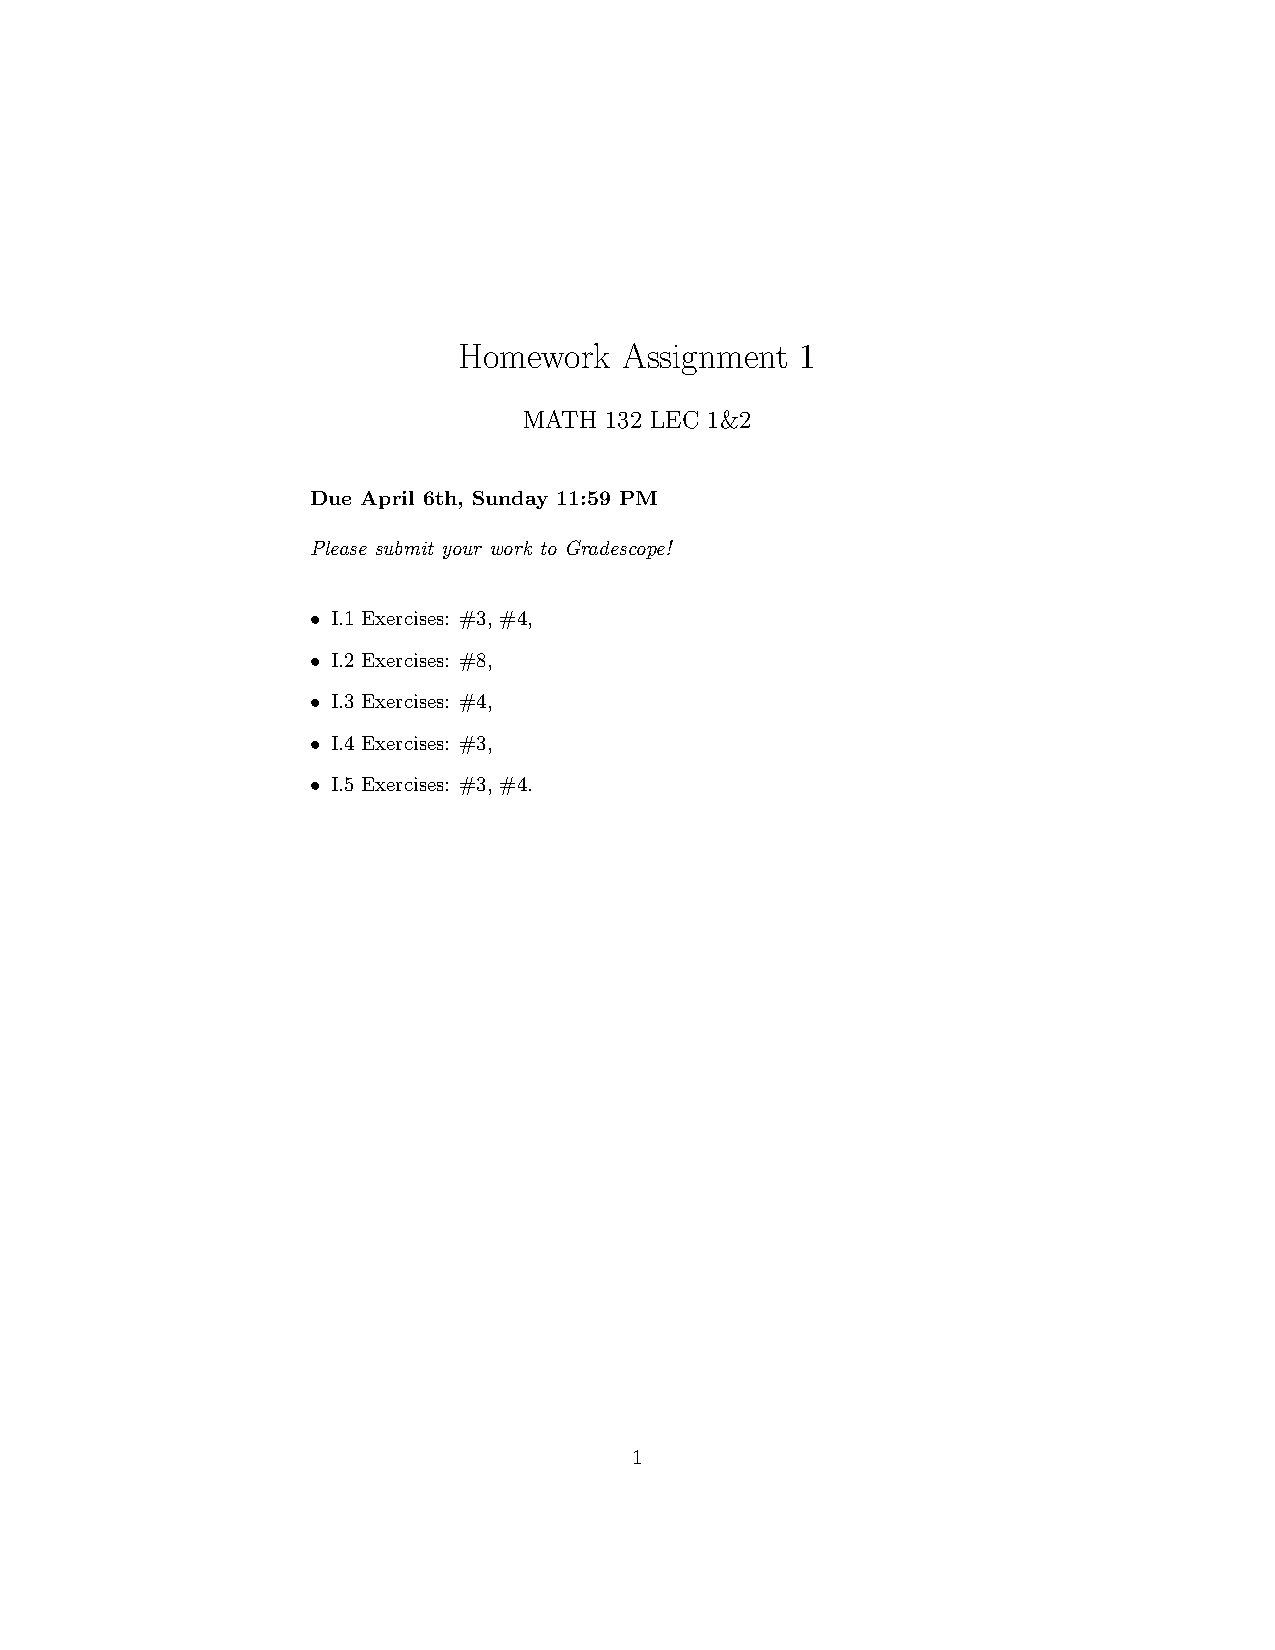
\includepdf[pages=-]{assignment.pdf}

\end{document}
